\chapter{Validation}
\label{chap:validation}

\vspace{-\baselineskip}

%##################################################################################################
\section{Chapter Overview}
%##################################################################################################

In order to evaluate the effectiveness of my approach, I undertook two separate pieces of validation work. The first piece involved quantifying the accuracy of the 3D feature identifiers presented in the previous chapter -- this was done by comparing their output to `gold standard' results produced manually in collaboration with a radiologist. The second piece involved validating the accuracy of my volume calculations. To do this, I first manually identified the liver, kidneys and spleen in a number of series and used my program to calculate their volumes in each case. The volume results were then correlated with known weights provided by the radiologist (bearing in mind that the densities of the organs in question are relatively uniform).

Both producing the gold standard results and making inter-result comparisons involved implementing special features for the purpose in \emph{millipede}. For the gold standard production, manual drawing tools were implemented to allow the user to draw round features of interest in the images. To make life easier for the user, the actual drawing was done using a \emph{Bamboo Fun} pen tablet (manufactured by Wacom) -- see Figure~\ref{fig:validation-pentablet-usage} -- although it would also have been possible to use a standard mouse. The inter-result comparisons were implemented as a dialog box allowing the user to compare multi-feature selections on a per-feature basis. The implementation of all the validation-specific features is discussed in Appendix~\ref{chap:appendixval}.

The validation work undertaken here forms an important part of the basis for the following chapter, in which I critically assess all the contributions claimed in the introduction.

%---
\stufigex{height=20cm}{validation/validation-pentablet-usage.png}{A typical user drawing round the right kidney using a `lasso' drawing tool similar to that found in common image-editing programs}{fig:validation-pentablet-usage}{p}
%---

%##################################################################################################
\section{Validation of 3D Feature Identifiers}
%##################################################################################################

To validate my 3D feature identifiers, I undertook four detailed case studies to test how well they worked on sets of slices from different series. An alternative approach of testing them on a larger number of series, but with less detailed individual analysis, would also have been possible, but in my view further work must be done on improving the robustness of the identifiers before such larger-scale validation really makes sense. The aim here is mainly to illustrate some of the areas in which the identifiers currently succeed or fail in order to highlight areas for further work.

For each case study, I produced a `gold standard' result by manually identifying the aorta, kidneys, liver, ribs, spinal canal, spine and spleen using the validation tools described in Appendix~\ref{chap:appendixval}. The resulting features were checked, and corrected where necessary, by Dr Zoe Traill, a Consultant Radiologist at the Churchill Hospital, Oxford. I then identified the same features using the automated multi-feature identifier. To perform a comparison, the gold standard result ($G$) and automated result ($A$) were used to construct three derivative multi-feature selections:
%
\begin{enumerate}
\item $A - G$, which contains the parts of the features that were identified by the automated identifier but should not have been.
\item $G - A$, which contains the parts of the features that were missed by the automated identifier.
\item $A \cap G$, which contains the parts of the features that were correctly identified.
\end{enumerate}
%
These were then used to calculate the Dice similarity coefficient for each feature, as described in \S\ref{sec:appendixval-featurecomparisons}, providing a quantitative measure of the extent to which the automated and gold standard results correspond.

%################################################
\subsection{Series BT-2, Slices $60$--$80$}
%################################################

\iffalse

Aorta

- Fairly good (Dice = 0.859), but automated result floods out into the left renal vein slightly due to a weak edge

Kidneys

- Only one kidney (other one is a huge tumour)
- Good (Dice = 0.949), only minor differences -- partly due to slight subjectivity of gold standard results, etc.

Liver

- Fairly good (Dice = 0.890)
- Missed the lateral segment of the left lobe -- because we find a single seed and flood from it, but the pieces are disconnected in the slices we've chosen
- Floods beyond the correct boundary in the direction of the aorta due to a weak edge

Ribs

- Reasonable (Dice = 0.773)
- But some ribs marked as spine -- because priority is currently given to the spine when there's a clash
  - Hence the table shows a high value for G - A

Spinal Canal

- Fairly good (Dice = 0.840)
- The automated result somewhat oversegments the canal -- why? (probably due to the fact that the regions within the spine only gradually get combined into a reasonable canal region that we could find, so that region ends up including all the bits inside the spine)
  - Hence the table shows a high value for A - G

Spine

- Good (Dice = 0.926)
- The automated result slightly oversegments the spine in places -- the top bit should be marked as rib
- It also tends to miss bits branching off the spine lower down -- why? (primarily because we're using branch node filtering rather than region flooding at present, but also because some of the bits sticking out are quite dark)

Spleen

- Fairly good (Dice = 0.853)
- The automated result contains some holes at the moment -- why? (primarily because it's an incipient identifier and we're not currently doing any flooding/hole filling)

\fi

TODO

%---
\begin{table}[p]
\begin{center}
\begin{tabular}{c|cccccc}
\footnotesize \textbf{Feature} & \footnotesize \textbf{Automated (A)} & \footnotesize \textbf{Gold (G)} & \footnotesize \textbf{A -- G} & \footnotesize \textbf{G -- A} & \footnotesize \textbf{A $\cap$ G} & \footnotesize \textbf{Dice} \\
\hline
\footnotesize Aorta & \footnotesize 13940 & \footnotesize 13973 & \footnotesize 1949 & \footnotesize 1982 & \footnotesize 11991 & \footnotesize 0.859 \\
\footnotesize Kidneys & \footnotesize 72142 & \footnotesize 73715 & \footnotesize 2915 & \footnotesize 4488 & \footnotesize 69227 & \footnotesize 0.949 \\
\footnotesize Liver & \footnotesize 180156 & \footnotesize 180693 & \footnotesize 19624 & \footnotesize 20161 & \footnotesize 160532 & \footnotesize 0.890 \\
\footnotesize Ribs & \footnotesize 22787 & \footnotesize 31125 & \footnotesize 1942 & \footnotesize 10280 & \footnotesize 20845 & \footnotesize 0.773 \\
\footnotesize Spinal Canal & \footnotesize 14451 & \footnotesize 11002 & \footnotesize 3758 & \footnotesize 309 & \footnotesize 10693 & \footnotesize 0.840 \\
\footnotesize Spine & \footnotesize 111889 & \footnotesize 113385 & \footnotesize 7634 & \footnotesize 9130 & \footnotesize 104255 & \footnotesize 0.926 \\
\footnotesize Spleen & \footnotesize 11841 & \footnotesize 15077 & \footnotesize 359 & \footnotesize 3595 & \footnotesize 11482 & \footnotesize 0.853 \\
\end{tabular}
\end{center}
\caption{A numeric comparison of the gold standard and automated results for the BT-2-60-80 feature identification case study. (All entries except those for the similarity coefficient are in voxels.)}
\label{tbl:validation-BT-2-60-80}
\end{table}
%---

%---
\begin{stusubfig}{p}
	\subfigure[Gold Standard Result]
	{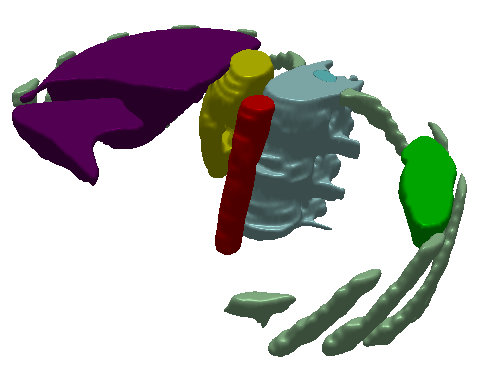
\includegraphics[width=.45\linewidth]{validation/validation-BT-2-60-80-goldstandard.png}}%
	%
	\hspace{4mm}%
	%
	\subfigure[Automated Result]
	{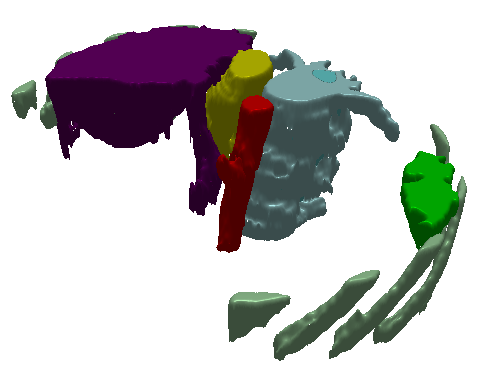
\includegraphics[width=.45\linewidth]{validation/validation-BT-2-60-80-target.png}}%
\caption{A visual comparison of the gold standard and automated results for the BT-2-60-80 feature identification case study}
\label{fig:validation-BT-2-60-80}
\end{stusubfig}
%---

\afterpage{\clearpage}
\newpage

%################################################
\subsection{Series SD-2, Slices $70$--$90$}
%################################################

\iffalse

Aorta

- Fairly good (Dice = 0.811)
- Floods out into a neighbouring blood vessel somewhat -- which one? same reason as for BT-2?

Kidneys

- Only one -- why? (can't remember)
- Good (Dice = 0.931)
- Automated result not quite as smooth -- why? (primarily an issue with the underlying segmentation)

Liver

- Good (Dice = 0.932)
- Doesn't miss a major part of the liver this time, because it's connected in the slices chosen
- Floods out towards the aorta -- why? (probably a weak edge)

Ribs

- Fairly good (Dice = 0.819)
- Picks up an erroneous bit which isn't a rib -- why? (probably because very bright in the image)
- Misses the odd bit which is a rib -- why? (check differences on scans)

Spinal Canal

- Fairly good (Dice = 0.862)
- Somewhat oversegmented -- for the same reasons mentioned for BT-2

Spine

- Good (Dice = 0.965), partly on account of this patient's notably high bone density
- Only minor differences, largely due to slight subjectivity of gold standard

Spleen

- Fairly good (Dice = 0.874)
- The automated result has missed a lot of the spleen -- why? (probably because I'm only finding a seed and not then flooding out from it)
- The automated result contains a lot of holes -- why? (probably because I'm not currently doing any hole filling)

\fi

TODO

%---
\begin{table}[p]
\begin{center}
\begin{tabular}{c|cccccc}
\footnotesize \textbf{Feature} & \footnotesize \textbf{Automated (A)} & \footnotesize \textbf{Gold (G)} & \footnotesize \textbf{A -- G} & \footnotesize \textbf{G -- A} & \footnotesize \textbf{A $\cap$ G} & \footnotesize \textbf{Dice} \\
\hline
\footnotesize Aorta & \footnotesize 12799 & \footnotesize 9848 & \footnotesize 3619 & \footnotesize 668 & \footnotesize 9180 & \footnotesize 0.811 \\
\footnotesize Kidneys & \footnotesize 93853 & \footnotesize 91324 & \footnotesize 7671 & \footnotesize 5142 & \footnotesize 86182 & \footnotesize 0.931 \\
\footnotesize Liver & \footnotesize 254945 & \footnotesize 231766 & \footnotesize 28156 & \footnotesize 4977 & \footnotesize 226789 & \footnotesize 0.932 \\
\footnotesize Ribs & \footnotesize 10331 & \footnotesize 10097 & \footnotesize 1962 & \footnotesize 1728 & \footnotesize 8369 & \footnotesize 0.819 \\
\footnotesize Spinal Canal & \footnotesize 15163 & \footnotesize 11655 & \footnotesize 3609 & \footnotesize 101 & \footnotesize 11554 & \footnotesize 0.862 \\
\footnotesize Spine & \footnotesize 84757 & \footnotesize 85430 & \footnotesize 2624 & \footnotesize 3297 & \footnotesize 82133 & \footnotesize 0.965 \\
\footnotesize Spleen & \footnotesize 46129 & \footnotesize 55049 & \footnotesize 1922 & \footnotesize 10842 & \footnotesize 44207 & \footnotesize 0.874 \\
\end{tabular}
\end{center}
\caption{A numeric comparison of the gold standard and automated results for the SD-2-70-90 feature identification case study. (All entries except those for the similarity coefficient are in voxels.)}
\label{tbl:validation-SD-2-70-90}
\end{table}
%---

%---
\begin{stusubfig}{p}
	\subfigure[Gold Standard Result]
	{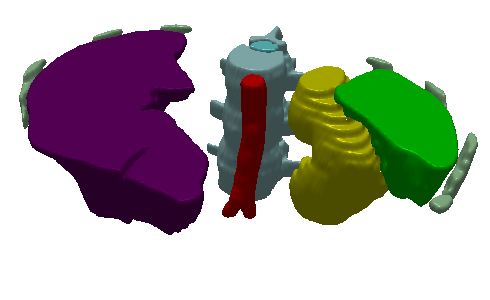
\includegraphics[width=.45\linewidth]{validation/validation-SD-2-70-90-goldstandard.png}}%
	%
	\hspace{4mm}%
	%
	\subfigure[Automated Result]
	{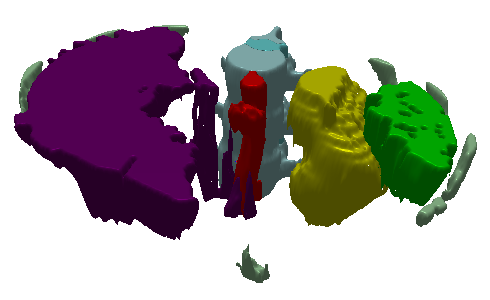
\includegraphics[width=.45\linewidth]{validation/validation-SD-2-70-90-target.png}}%
\caption{A visual comparison of the gold standard and automated results for the SD-2-70-90 feature identification case study}
\label{fig:validation-SD-2-70-90}
\end{stusubfig}
%---

\afterpage{\clearpage}
\newpage

%################################################
\subsection{Series MC-2, Slices $110$--$130$}
%################################################

\iffalse

Aorta

- Good (Dice = 0.908)
- Minor differences -- why? (primarily a result of the underlying segmentation)
- Overlapped by the liver, which has flooded out too far
  - The "easy" way to fix this is to unidentify as liver anything also marked as aorta, and then to find the connected components of the remaining liver bits and only keep sensible ones -- but that doesn't solve the problem in the general case

Kidneys

- Fairly good (Dice = 0.906)
- Flooded out a bit too far on the left kidney -- why? (check scans)
- The automated result is a bit smoother than the gold standard (not surprising, the slices are 5mm thick and the Laplacian smoothing is not perfect)

Liver

- Fairly good (Dice = 0.848)
- Flooded out much too far towards the aorta (completely overlapping it) -- why? (probably a weak edge)
- General outline isn't too bad
- Missed medial segment of left lobe -- why? (check scans)

Ribs

- Fairly good (Dice = 0.816)
- The automated result misses internal bits of ribs -- why?

Spinal Canal

- Good (Dice = 0.933)
- As ever, the automated result is slightly oversegmented -- see discussion for BT-2

Spine

- Good (Dice = 0.947)
- Minor differences are probably due to slight subjectivity of the gold standard (but check scans)

Spleen

- Fairly good (Dice = 0.898)
- As with SD-2, a certain amount of the spleen has been missed because not doing region flooding yet
- As with SD-2, contains a number of holes because not doing hole filling yet

\fi

TODO

%---
\begin{table}[p]
\begin{center}
\begin{tabular}{c|cccccc}
\footnotesize \textbf{Feature} & \footnotesize \textbf{Automated (A)} & \footnotesize \textbf{Gold (G)} & \footnotesize \textbf{A -- G} & \footnotesize \textbf{G -- A} & \footnotesize \textbf{A $\cap$ G} & \footnotesize \textbf{Dice} \\
\hline
\footnotesize Aorta & \footnotesize 15799 & \footnotesize 15036 & \footnotesize 1805 & \footnotesize 1042 & \footnotesize 13994 & \footnotesize 0.908 \\
\footnotesize Kidneys & \footnotesize 148065 & \footnotesize 137416 & \footnotesize 18698 & \footnotesize 8049 & \footnotesize 129367 & \footnotesize 0.906 \\
\footnotesize Liver & \footnotesize 492435 & \footnotesize 413475 & \footnotesize 108454 & \footnotesize 29494 & \footnotesize 383981 & \footnotesize 0.848 \\
\footnotesize Ribs & \footnotesize 33626 & \footnotesize 42708 & \footnotesize 2483 & \footnotesize 11565 & \footnotesize 31143 & \footnotesize 0.816 \\
\footnotesize Spinal Canal & \footnotesize 9924 & \footnotesize 9087 & \footnotesize 1054 & \footnotesize 217 & \footnotesize 8870 & \footnotesize 0.933 \\
\footnotesize Spine & \footnotesize 81483 & \footnotesize 79453 & \footnotesize 5247 & \footnotesize 3217 & \footnotesize 76236 & \footnotesize 0.947 \\
\footnotesize Spleen & \footnotesize 32048 & \footnotesize 36537 & \footnotesize 1240 & \footnotesize 5729 & \footnotesize 30808 & \footnotesize 0.898 \\
\end{tabular}
\end{center}
\caption{A numeric comparison of the gold standard and automated results for the MC-2-110-130 feature identification case study. (All entries except those for the similarity coefficient are in voxels.)}
\label{tbl:validation-MC-2-110-130}
\end{table}
%---

%---
\begin{stusubfig}{p}
	\subfigure[Gold Standard Result]
	{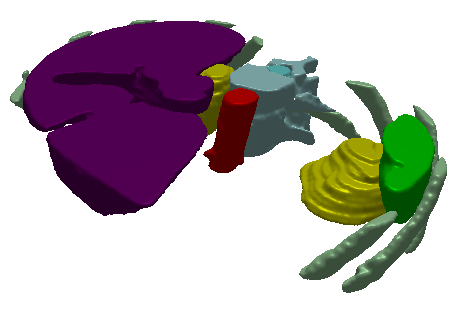
\includegraphics[width=.45\linewidth]{validation/validation-MC-2-110-130-goldstandard.png}}%
	%
	\hspace{4mm}%
	%
	\subfigure[Automated Result]
	{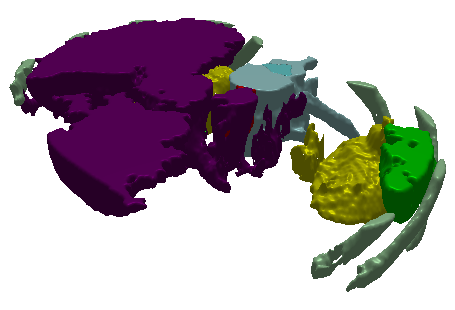
\includegraphics[width=.45\linewidth]{validation/validation-MC-2-110-130-target.png}}%
	%
	\hspace{4mm}%
	%
	\subfigure[Automated Result (excluding liver)]
	{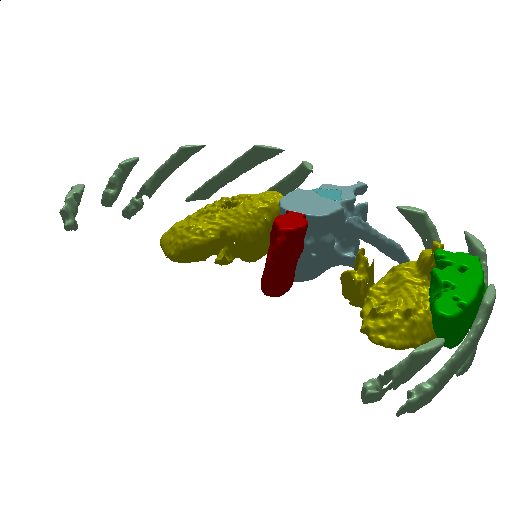
\includegraphics[width=.45\linewidth]{validation/validation-MC-2-110-130-target-noliver.png}}%
\caption{TODO}
\label{fig:validation-MC-2-110-130}
\end{stusubfig}
%---

\afterpage{\clearpage}
\newpage

%################################################
\subsection{Series EB-2, Slices $60$--$80$}
%################################################

\iffalse

Aorta

- Fairly good (Dice = 0.849)
- Automated result sticks out too far at the front -- why?
- Automated result is also missing bits in places -- where, and why? (check scans)

Kidneys

- Right kidney is good (Dice = 0.932)
- Left kidney is completely missed -- why? (primarily because of the tumour)
- Minor differences for right kidney are probably due to slight subjectivity of gold standard

Liver

- Good (0.948)
- Missing small bits of the left lobe -- why? (primarily because they're not connected in the slices chosen)
- Missing bits at the back -- why? (check scans)

Ribs

- Poor (Dice = 0.488)
- Segmenting lots of bits which aren't rib -- why? (probably because there are very bright bits on the images)

Spinal Canal

- Fairly good (Dice = 0.856)
- Again, somewhat oversegmented -- same reasons as for other series

Spine

- Good (Dice = 0.925)
- Automated result missing some of the bits sticking out -- why? (primarily because using branch node filtering instead of region growing, but also because some of the bits may be quite dark)
- Also segmenting bits it shouldn't -- which bits? (check scans)

Spleen

- Completely missed -- why? (check scans)

\fi

TODO (the left kidney is missed due to a tumour; the spleen is missed because there's not enough of it in the slices chosen (check this); the ribs are oversegmented because there are lots of unusually bright non-rib bits in EB-2)

%---
\begin{table}[p]
\begin{center}
\begin{tabular}{c|cccccc}
\footnotesize \textbf{Feature} & \footnotesize \textbf{Automated (A)} & \footnotesize \textbf{Gold (G)} & \footnotesize \textbf{A -- G} & \footnotesize \textbf{G -- A} & \footnotesize \textbf{A $\cap$ G} & \footnotesize \textbf{Dice} \\
\hline
\footnotesize Aorta & \footnotesize 10365 & \footnotesize 9416 & \footnotesize 1969 & \footnotesize 1020 & \footnotesize 8396 & \footnotesize 0.849 \\
\footnotesize Kidney (Right) & \footnotesize 47444 & \footnotesize 46918 & \footnotesize 3461 & \footnotesize 2935 & \footnotesize 43983 & \footnotesize 0.932 \\
\footnotesize Kidney (Left) & \footnotesize 0 & \footnotesize 36874 & \footnotesize 0 & \footnotesize 36874 & \footnotesize 0 & \footnotesize 0.000 \\
\footnotesize Liver & \footnotesize 160978 & \footnotesize 164834 & \footnotesize 6592 & \footnotesize 10448 & \footnotesize 154386 & \footnotesize 0.948 \\
\footnotesize Ribs & \footnotesize 10256 & \footnotesize 4959 & \footnotesize 6542 & \footnotesize 1245 & \footnotesize 3714 & \footnotesize 0.488 \\
\footnotesize Spinal Canal & \footnotesize 12387 & \footnotesize 9645 & \footnotesize 2958 & \footnotesize 216 & \footnotesize 9429 & \footnotesize 0.856 \\
\footnotesize Spine & \footnotesize 82721 & \footnotesize 85490 & \footnotesize 4946 & \footnotesize 7715 & \footnotesize 77775 & \footnotesize 0.925 \\
\footnotesize Spleen & \footnotesize 0 & \footnotesize 20179 & \footnotesize 0 & \footnotesize 20179 & \footnotesize 0 & \footnotesize 0.000 \\
\end{tabular}
\end{center}
\caption{TODO}
\label{tbl:validation-EB-2-60-80}
\end{table}
%---

%---
\begin{stusubfig}{p}
	\subfigure[Gold Standard Result]
	{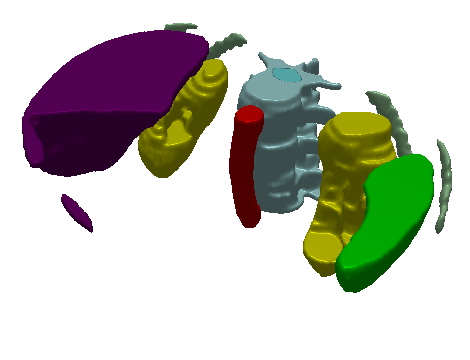
\includegraphics[width=.45\linewidth]{validation/validation-EB-2-60-80-goldstandard.png}}%
	%
	\hspace{4mm}%
	%
	\subfigure[Automated Result]
	{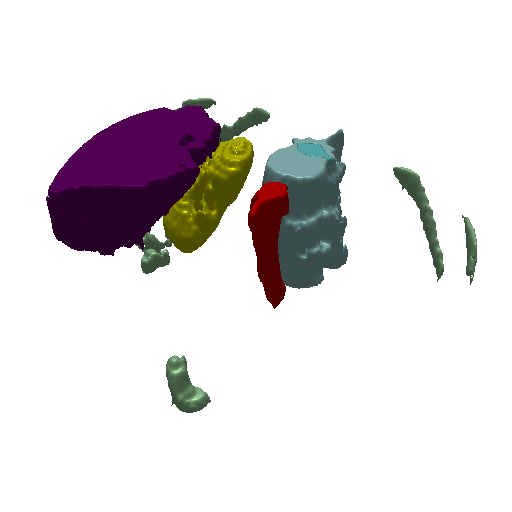
\includegraphics[width=.45\linewidth]{validation/validation-EB-2-60-80-target.png}}%
\caption{A visual comparison of the gold standard and automated results for the EB-2-60-80 feature identification case study}
\label{fig:validation-EB-2-60-80}
\end{stusubfig}
%---

\afterpage{\clearpage}
\newpage

%##################################################################################################
\section{Validation of Volume Calculations}
%##################################################################################################

TODO: \cite{woodard86}

%---
\begin{landscape}
\begin{table}[p]
\footnotesize
\begin{center}
\begin{tabular}{c|rrc|rrc|rr|rr}
\textbf{Patient} & \multicolumn{3}{|c|}{\textbf{Left Kidney}} & \multicolumn{3}{|c|}{\textbf{Right Kidney}} & \multicolumn{2}{|c|}{\textbf{Liver}} & \multicolumn{2}{|c}{\textbf{Spleen}} \\
& \emph{Mass} ($g$) & \emph{Vol.} ($\mathit{cm}^3$) & \emph{Cysts} $> 5\mathit{mm}$ & \emph{Mass} ($g$) & \emph{Vol.} ($\mathit{cm}^3$) & \emph{Cysts} $> 5\mathit{mm}$ & \emph{Mass} ($g$) & \emph{Vol.} ($\mathit{cm}^3$) & \emph{Mass} ($g$) & \emph{Vol.} ($\mathit{cm}^3$) \\
\hline
\hline
OX25 & 120 &  96.116 &            --- & 110 &  96.044 &                            --- & 1680 & 1468.657 & 110 & 105.568 \\
OX26 & 190 & 173.155 &            --- & 190 & 175.411 &                            --- & 1790 & 1752.384 &  40 &  32.879 \\
OX27 &  80 &  74.897 &              6 &  85 &  84.300 &                             12 & 1370 & 1156.192 & 140 & 121.837 \\
OX29 & 110 & 106.566 &            --- &  90 &  94.306 &                            --- & 1380 & 1323.991 & 170 & 121.665 \\
OX30 & 120 & 126.524 &         28, 27 & 120 & 113.079 &                              9 & 1819 & 1662.805 & 180 & 158.506 \\
OX31 & 200 & 175.163 &             14 & 170 & 153.155 &                            --- & 2120 & 1972.002 & 110 &  98.132 \\
OX33 & 120 & 111.776 &         12, 10 & 110 & 105.223 &                             10 & 1010 & 1042.976 & 110 &  98.362 \\
OX34 & 100 &  91.514 &            --- & 110 &  93.505 &                            --- &  880 &  792.150 &  70 &  65.271 \\
OX35 &  95 &  93.405 &             32 &  90 &  81.308 &                            --- & 1120 & 1091.544 &  45 &  35.542 \\
OX36 & 170 & 147.269 & 25, 19, 17, 10 & 140 & 126.720 & 15 ($\times$4), 10 ($\times$2) & 1660 & 1410.233 & 260 & 237.772 \\
OX37 & 160 & 132.421 &             23 & 140 & 110.786 &                            --- & 1210 & 1016.613 & 120 &  91.921 \\
OX38 & 126 & 114.638 & 24, 18, 13, 12 & 134 & 112.267 &                            --- & 1387 & 1501.876 & 196 & 203.940 \\
OX39 & 125 & 105.321 &            --- & 120 & 113.161 &                            --- & 1250 & 1212.430 & 120 & 104.221 \\
OX40 & 140 & 121.521 &            --- & 140 & 117.883 &                            --- & 1390 & 1297.704 & 110 &  78.971 \\
OX41 & 150 & 110.221 &            --- & 120 &  94.978 &                            --- & 1670 & 1577.043 & 150 & 124.464 \\
OX42 & 230 & 183.583 &            --- & 180 & 160.707 &                            --- & 1650 & 1565.364 & 100 &  85.891 \\
OX43 & 140 & 111.631 &            --- & 150 & 124.826 &                            --- & 1200 & 1066.671 & 190 & 165.091 \\
OX44 & 140 & 111.968 &            --- & 130 & 112.832 &                            --- & 1440 & 1344.238 & 130 &  83.531 \\
OX46 & 130 & 115.295 &            --- & 130 & 303.460 &                             80 & 1000 & 1020.945 &  90 &  81.773
\end{tabular}
\end{center}
\caption{TODO}
\label{tbl:validation-volcalc}
\end{table}
\end{landscape}
%---

%---
\stufigex{height=9cm}{validation/validation-volcalc-leftkidney.png}{TODO}{fig:validation-volcalc-leftkidney}{p}
%---

%---
\stufigex{height=9cm}{validation/validation-volcalc-rightkidney.png}{TODO}{fig:validation-volcalc-rightkidney}{p}
%---

%---
\stufigex{height=9cm}{validation/validation-volcalc-liver.png}{TODO}{fig:validation-volcalc-liver}{p}
%---

%---
\stufigex{height=9cm}{validation/validation-volcalc-spleen.png}{TODO}{fig:validation-volcalc-spleen}{p}
%---

\clearpage
\newpage

%##################################################################################################
\section{Chapter Summary}
%##################################################################################################

TODO
